\section{Tweet Author-Topic Model (with per-tweet topics)}
\begin{figure}[h]
\centering
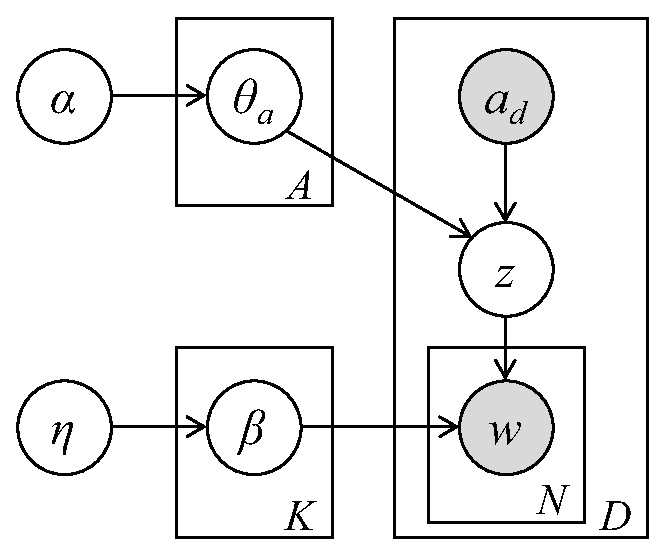
\includegraphics[width=0.4\linewidth]{TATM1}
\caption{Twitter Author-Topic Model with per-tweet topics.}
\label{fig:TATM1}
\end{figure}
This model is shown in figure \ref{fig:TATM1}. The only difference is we now assume a tweet has only one topic assignment, i. e. there is only one hidden variable $z$ per tweet or document. Our corresponding algorithm is shown in Algorithm \ref{alg:stoch_tatm1}. As we have only one local hidden variable per document we can't iteratively optimize it as it is done in the case of online LDA in \cite{Hoffman12}, where the local optimization is done by iteratively computing the sufficient statistics $\phi^k_{d,n}$ and the parameter of the document level topic distribution $\gamma_d$. We compute the sufficient statistics $\phi_{d,n}^k$ and then choose the topic $k^*$ which best explains the words in the current document. We then create an intermediate topic distribution for this author $\hat\gamma_a$ consisting of the virtual counts $\alpha$ and the observed counts $N$ in topic $k^*$. We then use this intermediate topic distribution $\hat\gamma_a$ to update author $a$'s topic distribution.